\documentclass[times, 10pt,twocolumn]{article} 
\usepackage{latex8}
\usepackage{times}
\usepackage{amsmath}
\usepackage{amsthm}
\usepackage{graphicx}
\usepackage{url}
\usepackage[T1]{fontenc}
\usepackage{color}
\usepackage{subfig}

\newtheorem{theorem}{Theorem}[section]

\newcommand{\comentario}[1]{}
\newcommand{\superscript}[1]{\ensuremath{^{\textrm{#1}}}}
\newcounter{notecounter}
\newcommand{\nota}[1]{\addtocounter{notecounter}{1}{\textcolor{red}{[nota
      \arabic{notecounter}: #1]}}}

\newcommand{\gnota}[1]{
  \addtocounter{notecounter}{1}
  \vspace{.5cm}
  \framebox{
    \begin{minipage}{0.95\linewidth}
      \textbf{nota \arabic{notecounter}:} #1
    \end{minipage}
  }\vspace{.5cm}}

\newcommand{\simul}{\textbf{RTSimul}} % Que criatividade. Mudar esse
% nome depois, urgente

\author{Alexandre Passos, George Lima, Jos\'e Augusto Matos Santos}
%\address{Universidade Federal da Bahia}
\title{On the Use of Hard and Soft Reservation Schemes in \\ Constant Bandwidth Servers}

\begin{document}

\graphicspath{{figs/}{data/}}

\maketitle

\begin{abstract}

  When scheduling soft real-time tasks it is usually a good idea to
  reserve fractions of the total bandwidth to each task (or task
  group). This reservation might be either \textbf{hard}, when under
  no circumstances a task might use some extra bandwidth, or
  \textbf{soft}, if there are some situations when it is allowed to do
  so. Usually, specially in the context of on-line adaptative systems,
  hard reservation is perceived to be more predictable, stricter and
  allowing faster adaptation. In this paper we argue that, perhaps
  surprisingly, allowing tasks to use some idle bandwidth shouldn't
  hurt their performance and reliability. To clarify our arguments we
  present the results of a few experiments performed on real-life and
  syntetic data sets using hard and soft variations of CBS, a commonly
  used reservation-based server.
  
\end{abstract}

\Section{Introduction}
\label{sec:introduction}

\textbf{Context}.  Real-time systems once structured as a set of
simple periodic hard tasks \cite{liu.ea73:scheduling} have become
reasonably complex. Nowadays such systems are often composed of hard
and soft real-time tasks, which can be both periodic and non-periodic.
Usual requirements of these modern real-time systems include not only
predictability but also responsiveness and adaptiveness. In this
context, reservation-based scheduling, \textbf{RBS} for short, has
successfully been applied to support such requirements
\cite{abeni.ea04:resource,mercer.ea94:processor,rajkumar.ea98:resource,sprunt.ea89:aperiodic,steffens.ea03:resource}.

RBS techniques are usually implemented by scheduling servers. A server
is a virtual task responsible for scheduling application tasks
assigned to it.  Each server $S_i$ can be defined by a processor
reservation tuple, $(Q_i,T_i)$, where $Q_i$ is called the server
capacity and $T_i$ the server period.  If a task (or group of tasks)
$\tau$ is assigned to a server $S_i$, $\tau$ has the right to use
$Q_i$ processor time within $T_i$ time units. Hence, servers can then
be scheduled as if they were simple periodic tasks.

On top of its conceptual simplicity, RBS has several interesting
properties \cite{steffens.ea03:resource}. From the scheduling
viewpoint it is worthing mentioning that: (a) RBS is a means of
ensuring temporal isolation since task execution can be controlled
within its reservation envelop
\cite{abeni.ea04:resource,mercer.ea94:processor,sprunt.ea89:aperiodic,spuri.ea96:scheduling};
(b) it is possible to implement hierarchical scheduling when a group
of tasks share the same server
\cite{davis.ea05:hierarchical,davis.ea08:investigation}; (c) it can be
used to improve flexibility, responsiveness and adaptiveness at the
scheduler level.  Such characteristics have motivated considerable
research in the area
\cite{abeni.ea99:adaptive,caccamo.ea00:capacity,caccamo.ea05:efficient,oliveira.ea08:dynamic,oliveira.ea09:dynamic,lin.ea05:improving}.
In this paper we aim at better characterizing the performance of two
reservation schemes commonly implemented in real-time systems.

\textbf{Focus}.  A reservation scheme is \textbf{hard} if a server
$S_i = (Q_i,T_i)$ cannot be scheduled run for more than $Q_i$ time
units within any time interval of $T_i$ units even if there is idle
processor time available. On the other hand, a \textbf{soft} scheme
allows $S_i$ to execute beyond its reservation as long as system
schedulability is not compromised. Often the decision of implementing
one of these schemes arises. One of the widely known implementations
of soft RBS scheme in EDF scheduled systems is the Constant Bandwidth
Servers (\textbf{CBS}) \cite{abeni.ea04:resource}.  Due to the number
of other scheduling mechanisms based on CBS
\cite{abeni.ea05:qos,caccamo.ea00:capacity,caccamo.ea05:efficient,lipari.ea00:greedy},
we chose it as a case study in this paper.

According to the CBS rules, a constant bandwidth $u_i = Q_i/T_i$ is
allocated to each server $S_i = (Q_i,T_i)$, where $Q_i$ is called
hereafter the maximum server budget. The budget of each server $S_i$
is consumed as its jobs are executed. To guarantee that the server
obeys its utilization limit, the deadline of $S_i$ is postponed by
$T_i$ every time its budget is depleted.  Its full budget $Q_i$ is
also restored when its deadline is updated.  Deadline postponements
make it possible to implement the soft reservation scheme but brings
about a potential side effect: an overloaded server may have its
deadline postponed too often making its relative priority too low.
This problem may be avoided by implementing a hard reservation version
of CBS \cite{buttazzo05:soft}, which waits until the current server
deadline to recharge the server budget.  Nonetheless, it is still to
be checked whether soft or hard CBS performs better.

\textbf{Related work}. There is extensive research on comparing RBS
techniques.  Some of them have been on fixed-priority scheduling
\cite{bernat.ea99:new,bernat.ea02:multiple,davis.ea05:hierarchical,davis.ea95:dual}.
In the field of dynamic scheduling, CBS has been compared to several
other approaches \cite{spuri.ea96:scheduling}.  Techniques to
reclaiming spare capacity of CBS have also been reported, bringing in
comparative studies on their performance
\cite{caccamo.ea00:capacity,lin.ea05:improving}. To the best of our
knowledge these comparative studies have considered only the soft
version of CBS, though.  The work by Rajkumar et
al. \cite{rajkumar.ea01:resource} illustrates the use of hard and soft
versions of a fixed-priority RBS using a very simple task set.

\SubSection{Contributions of this paper}
\label{sec:contr-this-paper}

We report a comprehensive comparative study on the performance of
CBS. The reported evaluation puts into perspective the perceived
characteristics of its hard and soft reservation schemes.  By
benchmarking these two CBS versions in a simulation environment, they
are systematically compared against each other.  Since the use of CBS
has extensively been reported and one usually chooses arbitrarily
between these two versions
(e.g. \cite{abeni.ea99:adaptive,abeni.ea05:qos}), the results reported
here can better subsidize their implementation decisions.  The
reported study was carried out making use of the real-time scheduling
simulator \simul{}, implemented in Pyton. Although there are other
simulation tools \nota{citar simTools}, implementing this simulator
ourselves allowed us to easily tune it to our specific requirements.

\SubSection{Structure of this paper}
\label{sec:structure-this-paper}

Section \ref{sec:simul-envir} describes the system model and the
simulation environment.  In order to give a wide picture of the
simulated scheduling mechanisms, we conducted the evaluation taken
into consideration several metrics and different simulation
scenarios. Results from the simulation are discussed in Section
\ref{sec:simulation-results} while in Section \ref{sec:conclusion} our
final comments are given.

\Section{Simulation Environment}
\label{sec:simul-envir}

To perform the experiments presented in this paper we implemented
\simul{}, a simple python-based simulator for real-time scheduling
algorithms. Its source code, the data files used in this paper and
instructions to reproduce our results are available in
\url{http://github.com/jamsjr/hard-versus-soft/tree/master}. \simul{}
implements a basic EDF scheduler and, on top of it, runs both hard
real-time periodic tasks and bandwidth sharing servers. These servers
can be either traditional CBS servers \cite{abeni.ea98:integrating} or
a hard reservation adaptation of the CBS algorithm, as described in
\cite{buttazzo05:soft}. Soft real-time tasks running on these servers
either have their execution times sampled from a probability
distribution or follow traces generated from a modified version of
mplayer that reports the start time and decoding cost for each frame
in a high-resolution video. The same time unit standard was used for
both the video trace and the synthetic task sets so that all presented
measurements are platform-independent.

All the simulations performed in this paper share a common
set-up. There is a periodic hard real-time task running in the
background, with fixed period (\nota{x}), execution cost (\nota{y})and
deadline (\nota{z}).  There is also one soft real-time server,
implementing either hard or soft reservation schemes.  This server
will be monitored during the simulation so that both reservation
schemes can be compared against each other. More complex simulations,
involving more servers and tasks, were also tested. In both complex
and simple simulation set-ups, the behavior of the reservation schemes
was shown to be similar. Hence, we chose to present here the simplest
simulation set-up for the sake of data analysis.  Several
configurations of this set-up were considered.

\SubSection{Simulation Configurations}
\label{sec:configurations}

In order to simulate several application semantics, we consider four simulation parameters: 
\begin{description}
\item Discard/not discard expired tasks. For some applications it is
  better to discard tasks when they miss their deadlines while for
  other ones tasks are kept executing after their expired deadlines.
\item High/low execution cost variance. Execution cost variance plays
  an important role when tuning the server parameters. Server
  capacities are usually adjusted to the mean execution cost
  value. Varying this parameter we verify the behavior of the
  reservation schemes for these two extreme scenarios.
\item Overloaded/not overloaded system. We consider a system
  overloaded when its tasks demand more than 100\% of CPU.
\item Overloaded/not overloaded server. A server $S$ is overloaded
  when its utilization $u = Q/T$ is not enough to serve the
  tasks it is serving.
\end{description}

Considering all combination of these four parameters leads to 16
distinct configurations. In several of them the behaviors of both
reservation schemes were found to be equivalent.  We will present here
only the results for those which showed difference in performance.
The metrics we use to measure these differences in performance are
response time, wait time and deadline miss ratio.

\Section{Simulation Results}
\label{sec:simulation-results}

Section \ref{sec:charact-server-load} first presents some individual
scenarios we considered relevant for our experiments. As mentioned in
section \ref{sec:configurations}, not all configurations led to a
performance difference. Section \ref{sec:noDifference} presents some
comments on the reasons for this behavior. Finally, section
\ref{sec:indiv-simul-results} describes the results that highlight any
differences in performance between the hard and soft reservation
schemes.

\SubSection{Characterizing the server load}
\label{sec:charact-server-load}

Four distinct application loads (L1-L4) were considered by varying the
execution cost distributions.  For the sake of data analysis, it is
interesting to observe how hard and soft reservation schemes behave
with more controlled load distributions. This is the goal of loads
L1-L3, which takes synthetic generated data. The data correspond to
execution times of jobs to be served during $9,000$ time units of
simulation.  The inter-arrival time of these jobs were kept constant
and equal to one time unit.  The load L4 was taken by a movie trace
and was used to represent more realistic soft-real time data. The
characteristics of these four loads are given below.

\begin{description}
\item L1: Constant mean execution time and low variance. Job execution
  costs were generated during the simulation time, set to $9,000$ time
  units, according to a normal distribution with mean $0.6$ and (low)
  variance equal to $0.01$. In other words, the execution cost of each
  job to be served follows $\mathcal{N}(0.6,0.01)$. This scenario can
  be seen in Figure \ref{fig:plotl1}
\item L2: Variable mean execution time and low variance.  In order to
  simulate controlled variation of execution times, two values for the
  mean execution time were considered, taken from
  $\mathcal{N}(0.6,0.01)$ and $\mathcal{N}(0.4,0.01)$. During the time
  intervals $[0;3,000)$ and $(6,000;9,000]$ data from the former
  distribution while the latter were used to generate data for
  interval $[3,000;6,000]$. This simulates scenarios were application
  demands different execution times during certain phases of its
  execution. This scenario is displayed in Figure \ref{fig:plotl2}
\item L3: Constant mean execution time and variable variance.  Another
  simulated scenario considered two simulation intervals, $[0;4,500)$
  and $[4,500;9,000)$.  The execution costs for these intervals
  followed two distributions, $\mathcal{N}(0.6,0.01)$ and
  $\mathcal{N}(0.6,0.1)$. This scenario is displayed in Figure
  \ref{fig:plotl3}
\item L4: A movie trace. The costs are shown in Figure
  \ref{fig:plotl4}. The values in the graph correspond to the decoding
  times using the \texttt{mplayer} media player for the Eve movie. In
  this trace jobs arrive with a mean period of 0.072 time units and
  mean costs of 0.0064 time units. This trace is considered for the
  purpose of testing the behavior of both reservation schemes with a
  real-life data set.
\end{description}

\begin{figure}[h!t]
  \centering
  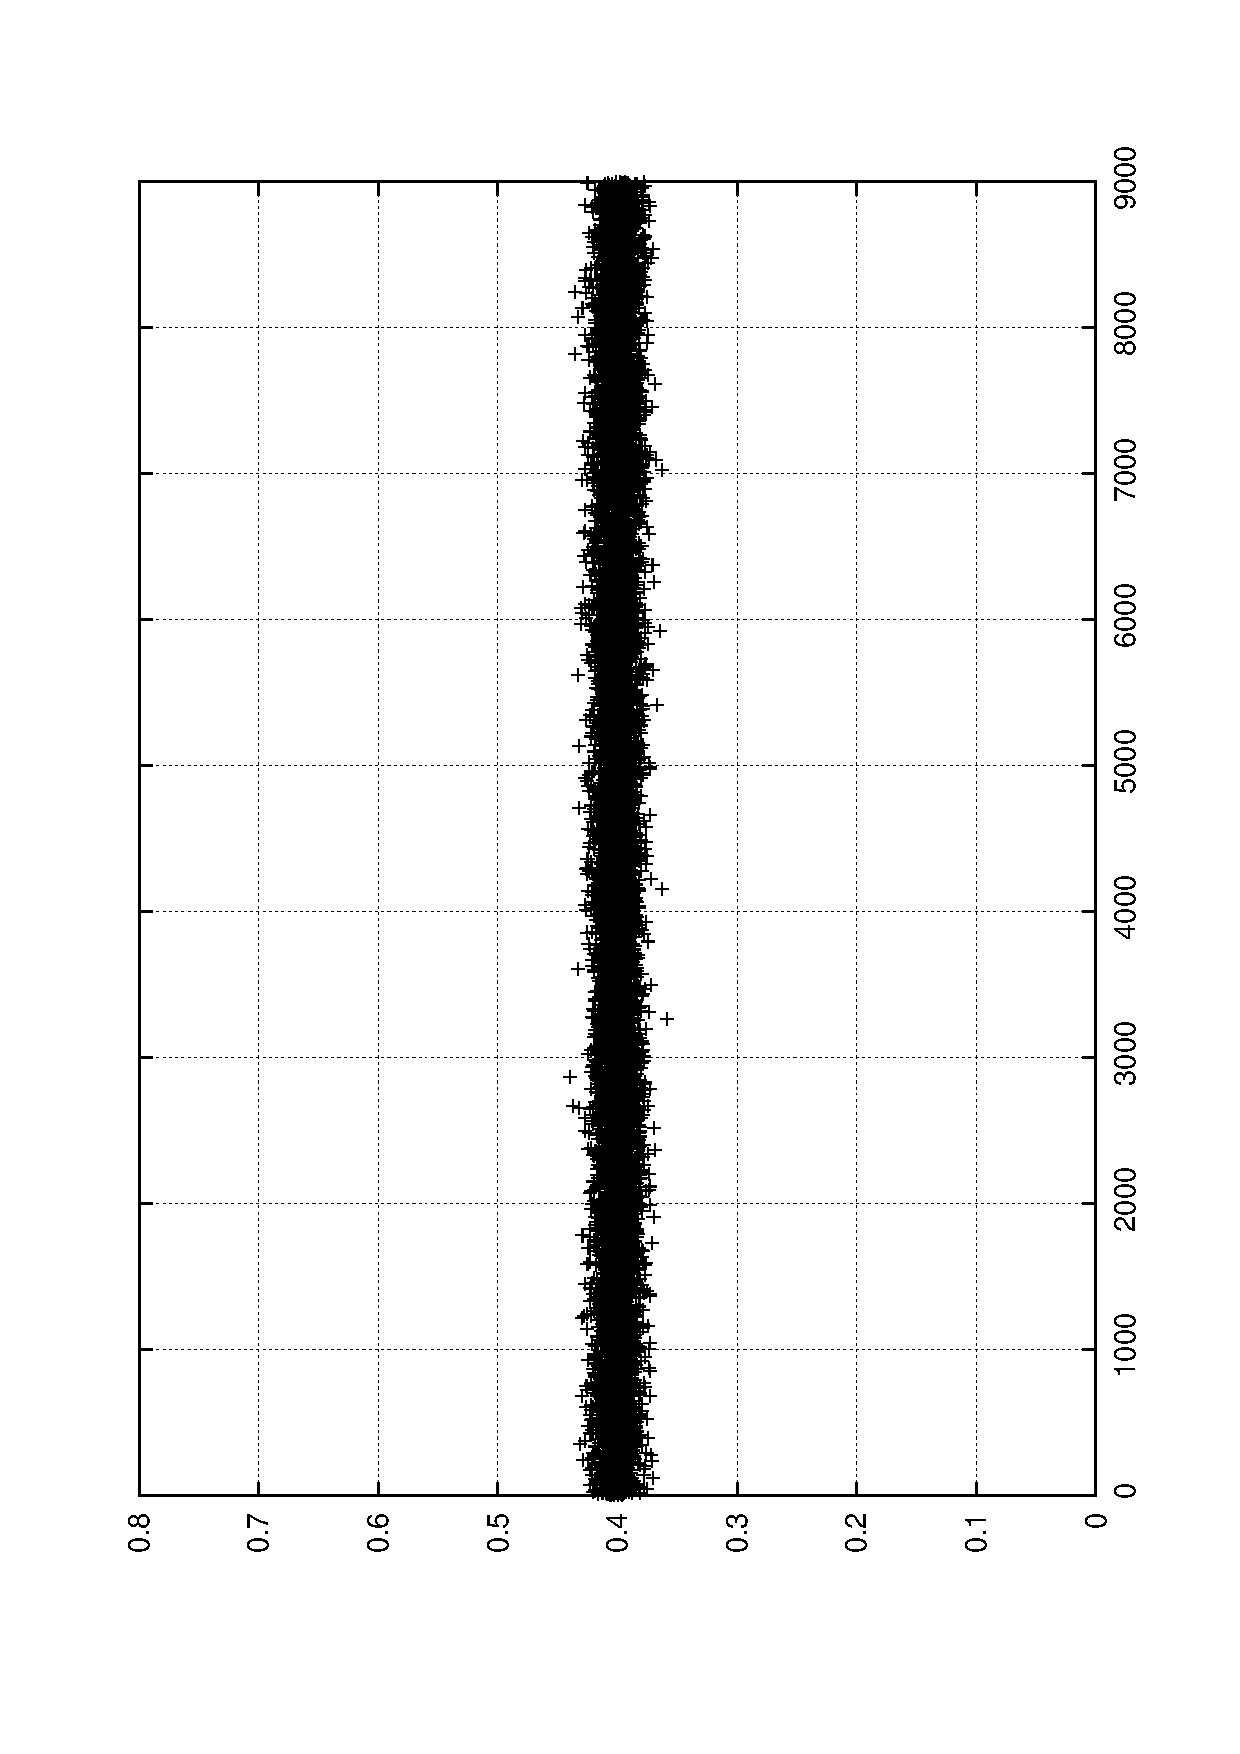
\includegraphics[scale=0.33]{trace-normal}
  \caption{Execution cost distribution for the scenario L1.}
  \label{fig:plotl1}
\end{figure}

\begin{figure}[h!t]
  \centering
  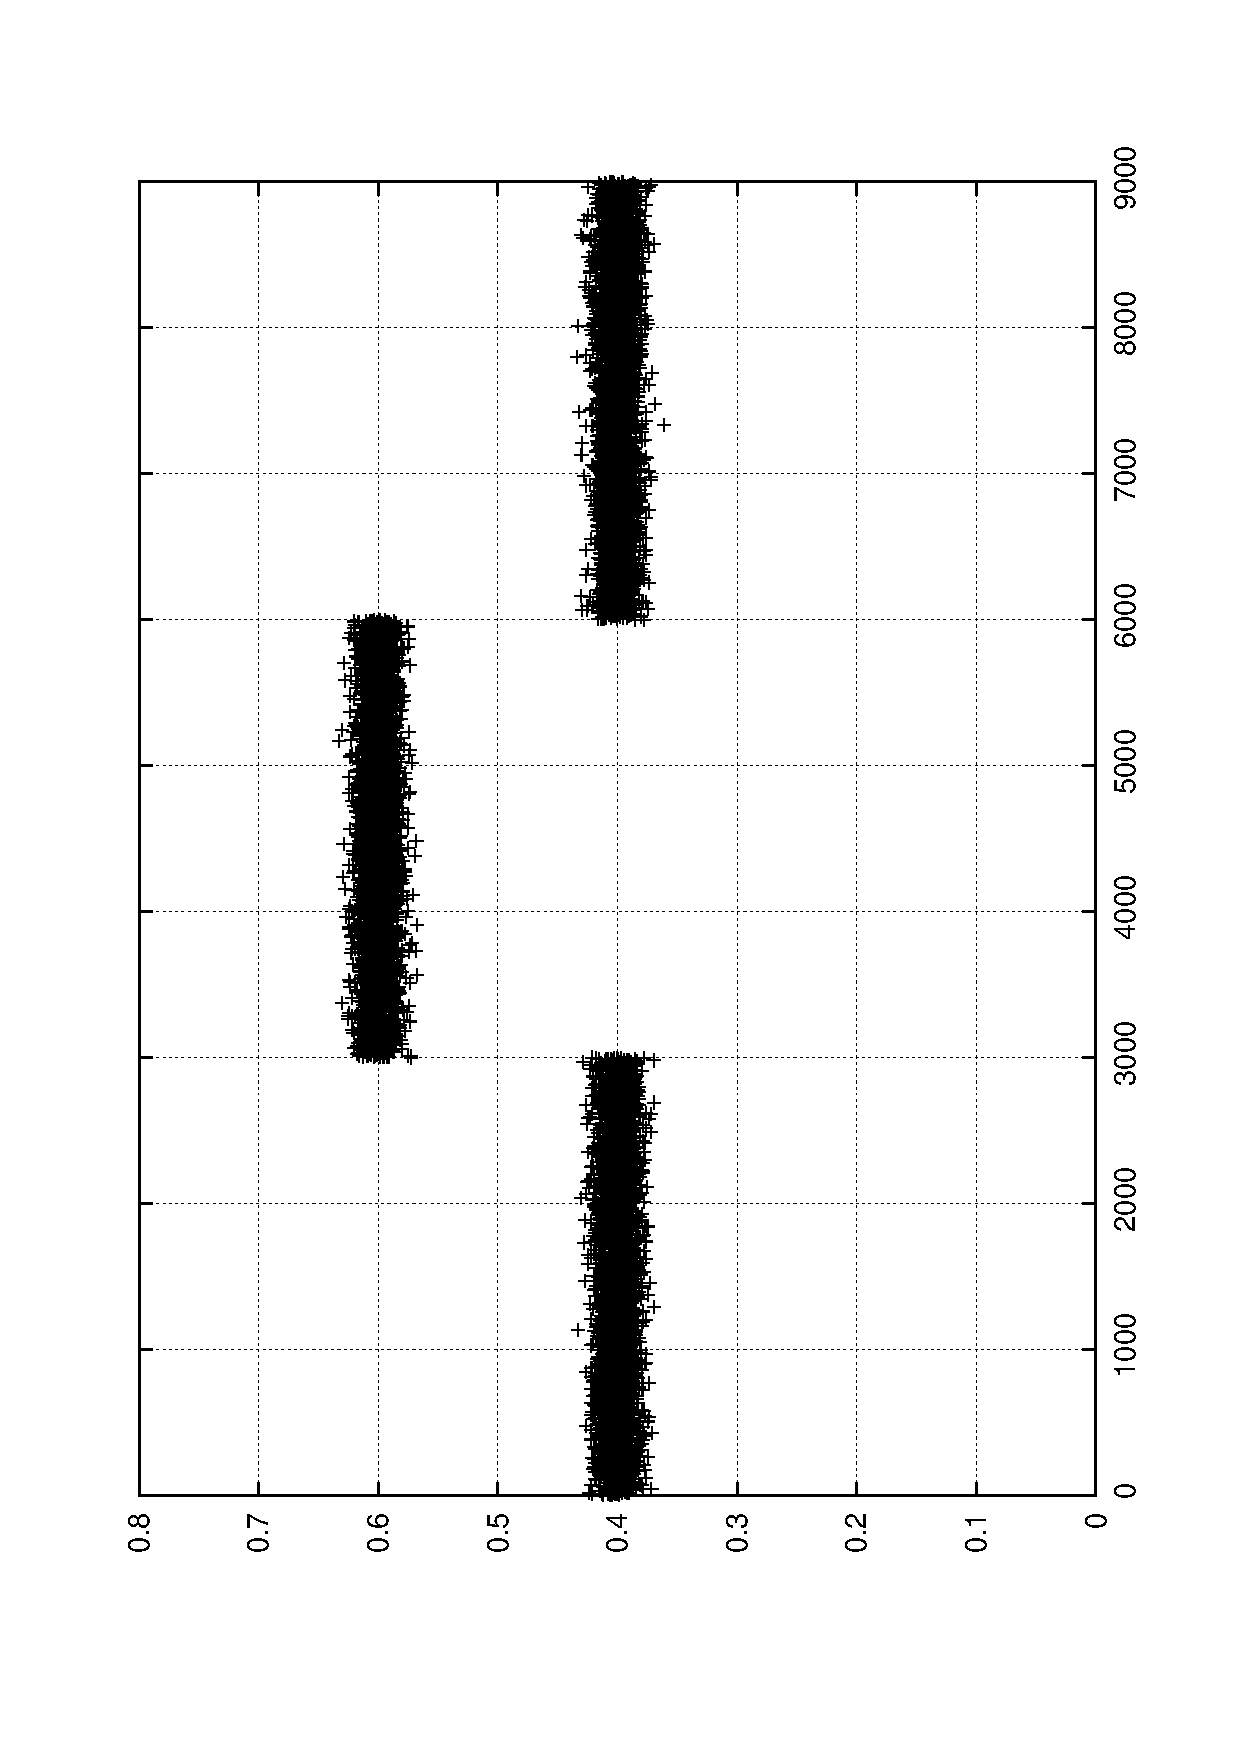
\includegraphics[scale=0.33]{trace-trifasico}
  \caption{Execution cost distribution for the scenario L2.}
  \label{fig:plotl2}
\end{figure}

\begin{figure}[h!t]
  \centering
  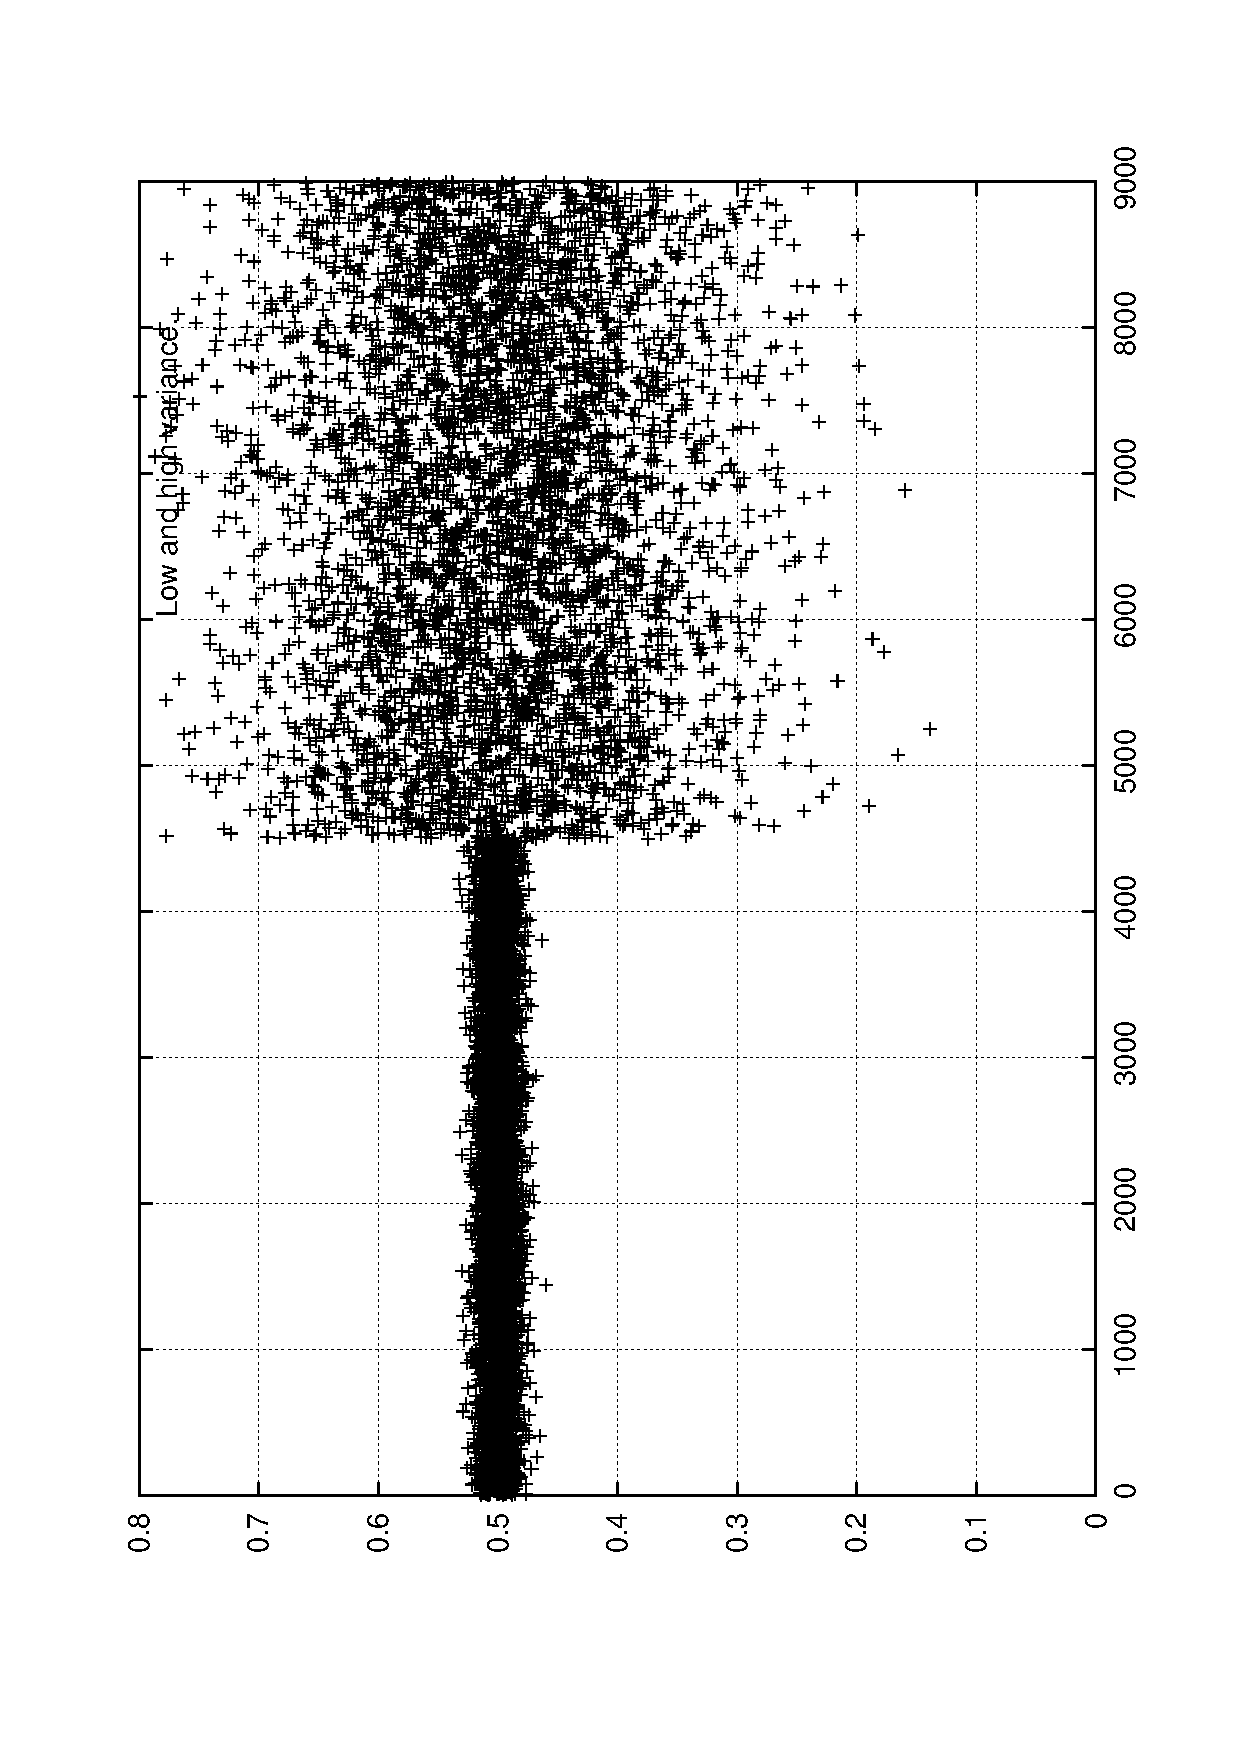
\includegraphics[scale=0.33]{trace-variance}
  \caption{Execution cost distribution for the scenario L3.}
  \label{fig:plotl3}
\end{figure}

\begin{figure}[h!t]
  \centering
  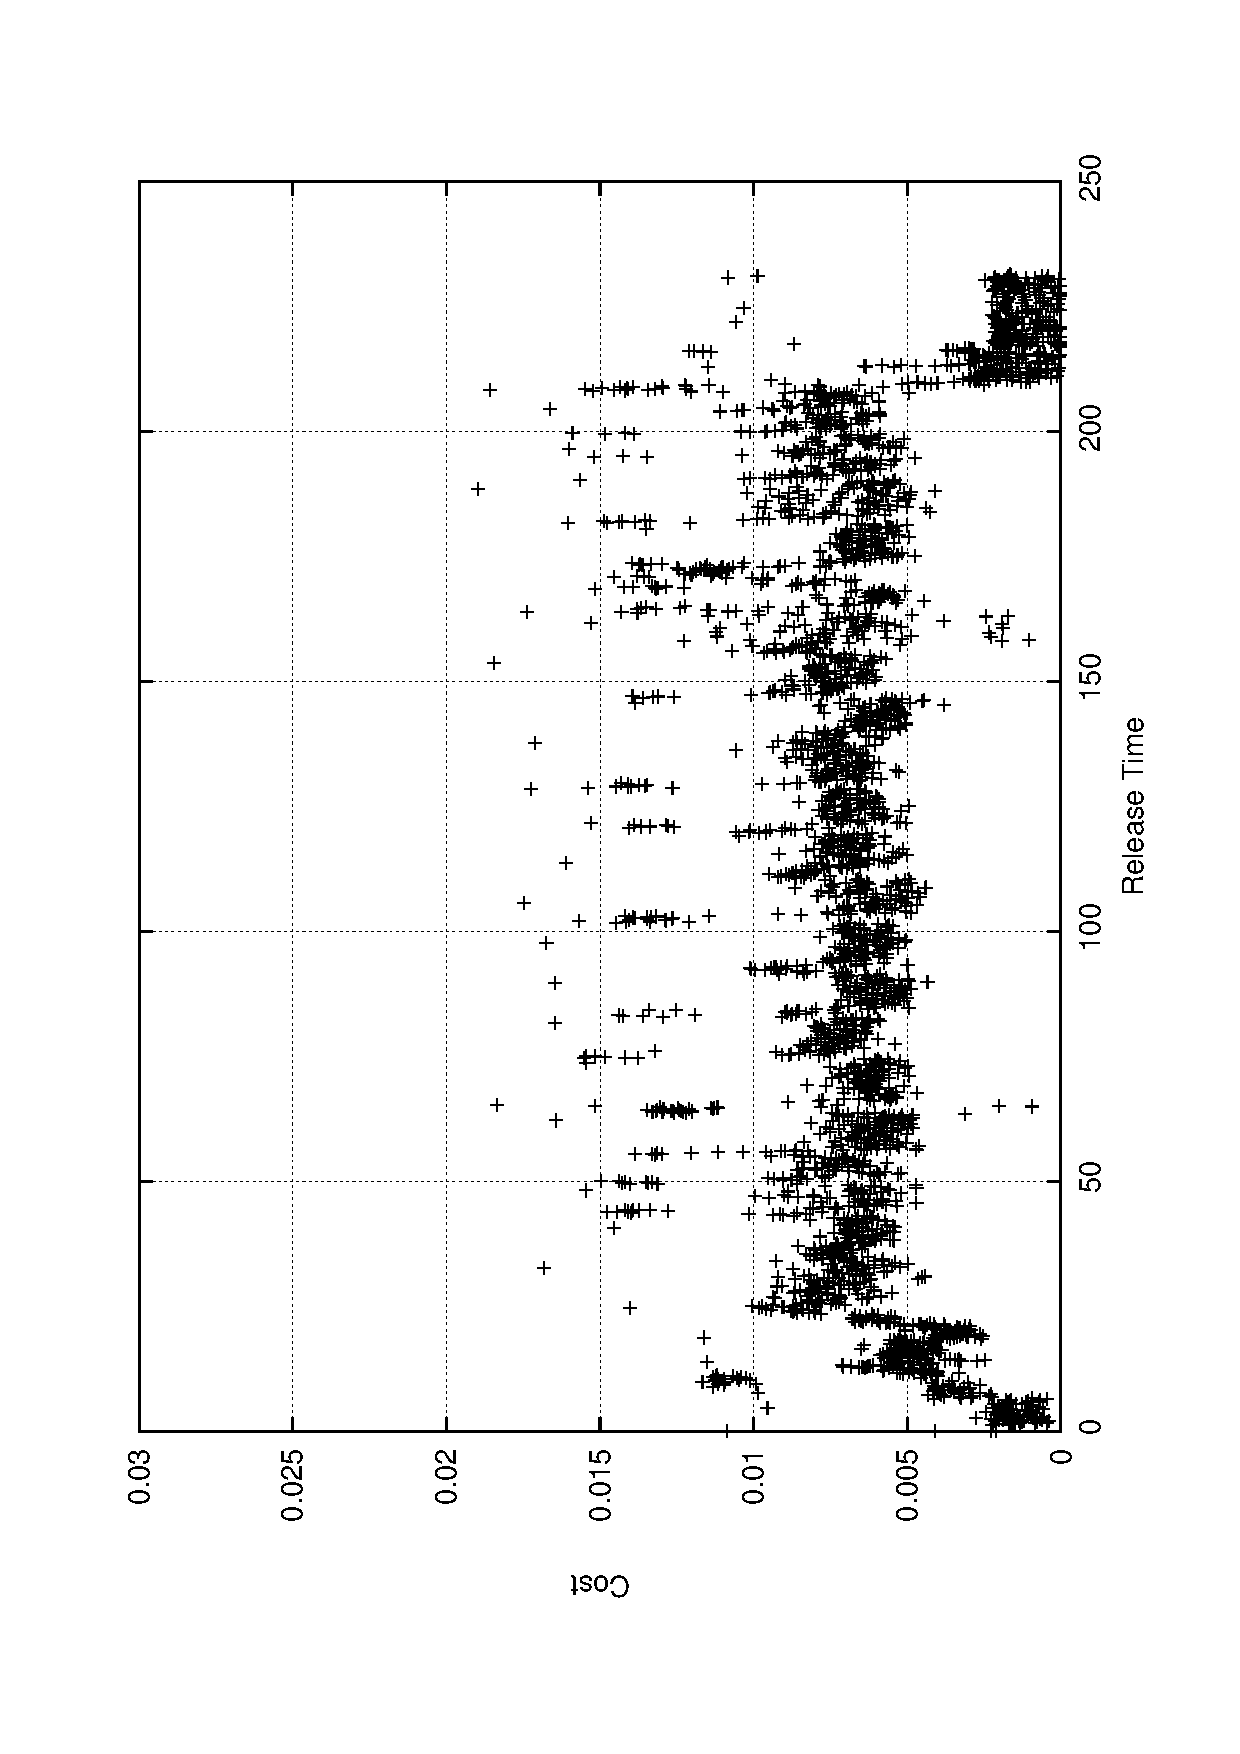
\includegraphics[scale=0.33]{trace-eve}
  \caption{Execution cost distribution for scenario L4.}
  \label{fig:plotl4}
\end{figure}

In the following subsections the found results for loads L1-L4 are presented. 

\SubSection{Scenarios With Equivalent Reservation Performance}
\label{sec:noDifference}

Hard and soft reservation schemes shown equivalent performance in all
configurations.  In situations when expired tasks are not discarded,
the system is constantly overloadedloaded or the server is underloaded
both reservation schemes performed equivalently. The explanation for
this behavior is given below.

\subsubsection{Discarding expired tasks}
\label{sec:disc-expir-tasks}

Consider a server $S = (Q,T)$ and that at time $t$ there is a
execution cost of $C$ to be served.  Since expired tasks are
discarded, both hard and soft reservation servers will finish in at
least $\lfloor C/Q \rfloor T$ time units.  The only possible
difference is that a soft reservation server might spend this budget
before a hard reservation server can. In that case, the soft
reservation server may suffer some deadline postponments, but can
never finish executing a given job after an equivalent hard
reservation server.

Hence, in general, not discarding expired tasks makes soft and hard
reservation completely equivalent. 

\subsubsection{Overloaded system}
\label{sec:system-load}

When the system is always perfectly dimensioned or overloaded (there
is no system idle time) both reservation schemes are equivalent. This
is so because the soft server can only postpone its deadline to get
extra budget when there is free system time. Even if a soft
reservation server does exaust its budget before its deadline, a
system under high load will usually have other higher-priority tasks
running and hence stopping the soft reservation server from using its
extra budget until the time gets closer to the server deadline (and by
then an equivalent hard reservation server would already be able to
use its budget).

\subsubsection{Underloaded server}
\label{sec:server-load}

Another scenario that does not highlight any differences between hard
and soft reservation is when the server load is low enough that there
is always free budget upon completing a task. In these situations both
hard and soft reservation mechanisms are equivalent, because, as less
budget is needed per server period than the server capacity, the will
be usually no budget exhaustion.\nota{george: Nao faz sentido dizer
  que nao ha budget exhaustion. Tem que formular melhor esta
  explicacao. Eu acrescentei algo a frase, mas ainda assim, continua
  sem sentido. alexandre: está melhor?}

\SubSection{Scenarios With Unequivalent Performance}
\label{sec:indiv-simul-results}

Exploring all possible situations that might highlight any differences
between soft and hard reservation is unpractical, so we chose a few
representative cases, already described in section
\ref{sec:configurations} as L1, L2, L3 and L4. Configuration L1
supposedly highlights how the servers are expected to behave under
reasonable conditions. L2 is designed to see how the servers adapt to
varying costs, and L3 varying variance. L4, on the other hand, is a
real-life example, that reproduces behavior observed under the other
configurations, as expected. Table \ref{tab:summary} summarizes the
results.

\begin{table*}[t]
  \centering
  \begin{tabular}[t]{rrrrr} \hline
    \textsc{Scenario} & \textsc{Reservation model} & \textsc{Mean
      response time} & \textsc{Mean waiting time} & \textsc{Deadline
      miss ratio (\%)} \\ \hline
    L1 & Soft & 0.51   & 0.25   & 5.4  \\
    L1 & Hard & 0.56   & 0.41   & 59.8 \\
    L2 & Soft & 0.48   & 0.17   & 14.4 \\
    L2 & Hard & 0.44   & 0.31   & 37.5 \\
    L3 & Soft & 0.57   & 0.24   & 5.1  \\
    L3 & Hard & 0.58   & 0.41   & 59.4 \\
    L4 & Soft & 0.0065 & 0.0022 & 0.1  \\
    L4 & Hard & 0.035  & 0.022  & 24.5 \\ \hline    
  \end{tabular}
  \caption{Result summary}
  \label{tab:summary}
\end{table*}

\begin{figure*}[t]
  \centering
  \subfloat[Soft reservation.]{
    \includegraphics[scale=0.33]{rthisto1}
    \label{fig:soft-rth}
  }
  \subfloat[Hard reservation.]{
    \includegraphics[scale=0.33]{rthisto2}
    \label{fig:hard-rth}
  }
  \caption{Response time histograms for scenario L1.}
  \label{fig:rth}
\end{figure*}

\begin{figure*}[t]
  \centering
  \subfloat[Soft reservation.]{
    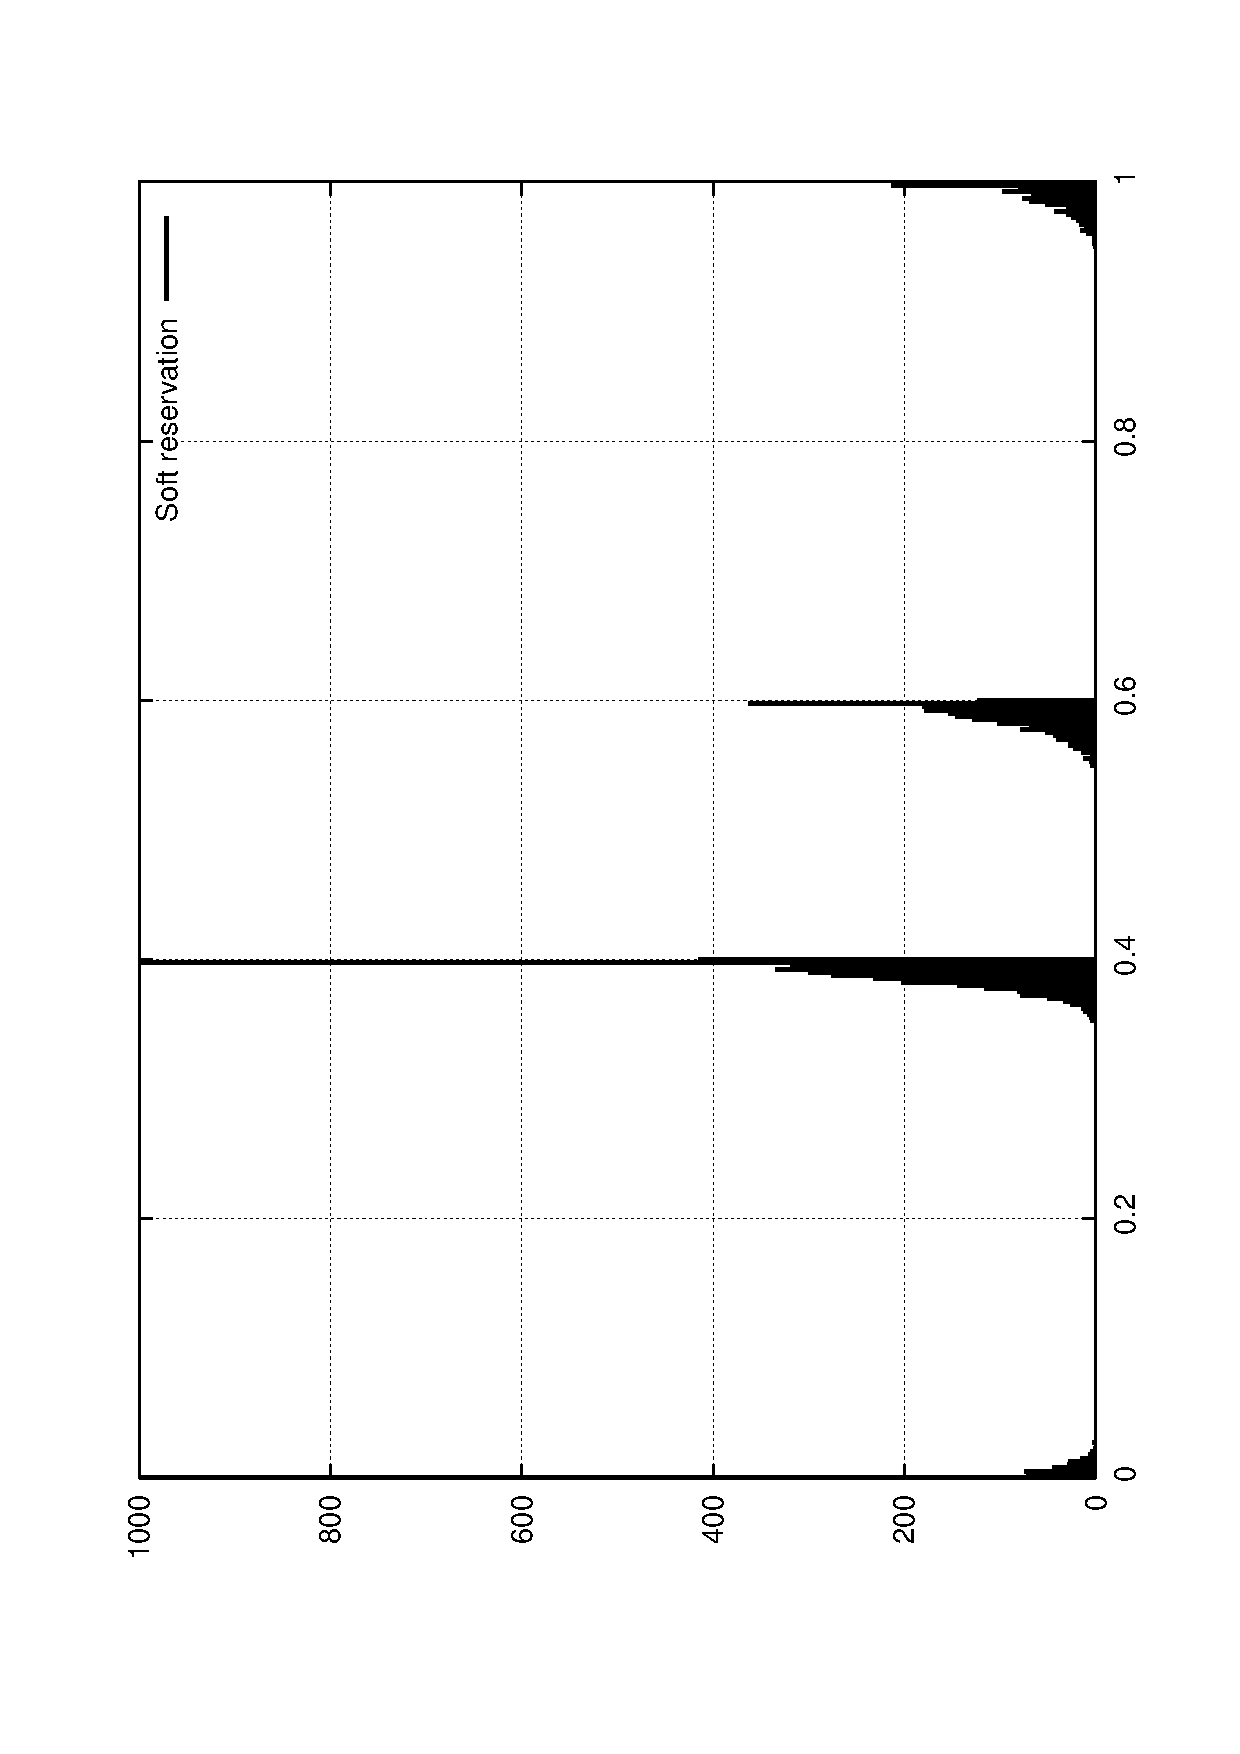
\includegraphics[scale=0.33]{dthisto1}
    \label{fig:soft-dth}
  }
  \subfloat[Hard reservation.]{
    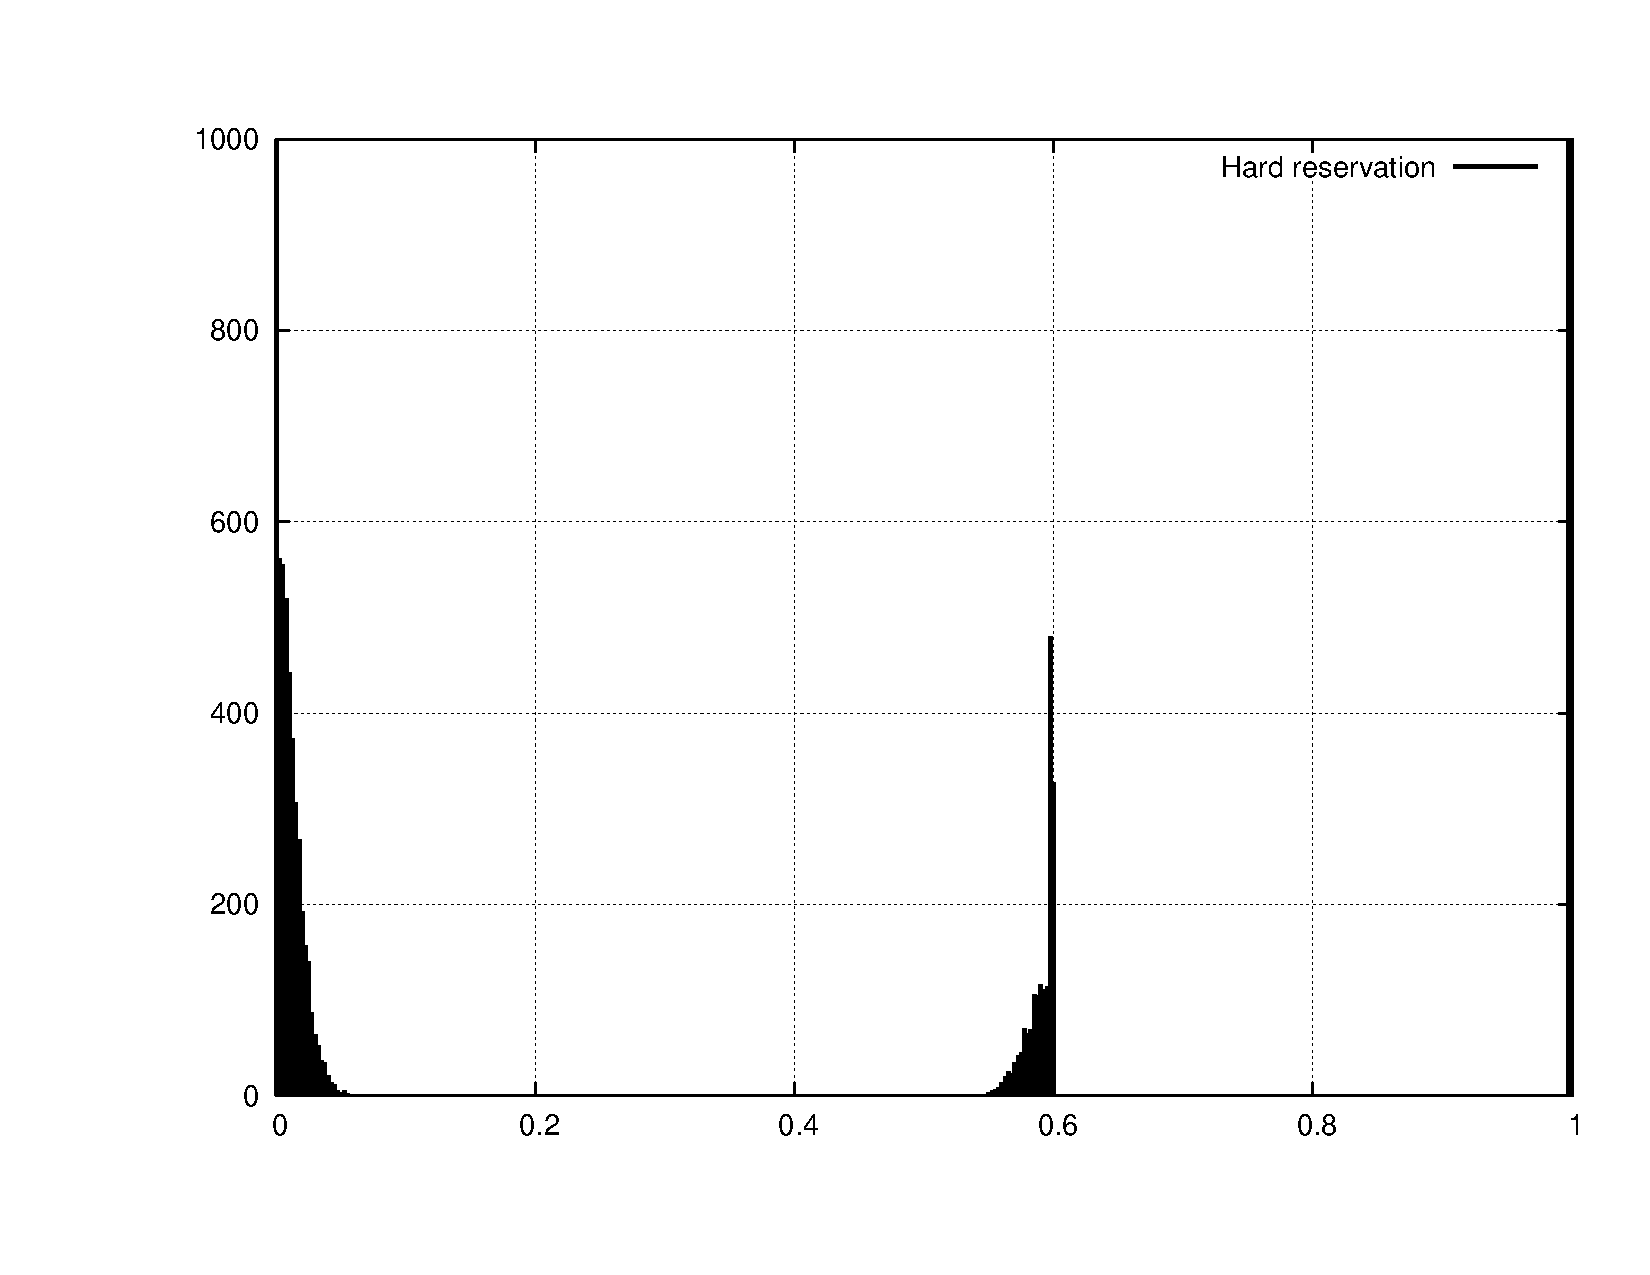
\includegraphics[scale=0.33]{dthisto2}
    \label{fig:hard-dth}
  }
  \caption{Wait time histograms for scenario L1.}
  \label{fig:dth}
\end{figure*}

For a general idea of how soft and hard reservation behave we have
used the costs in scenario L1. Figures \ref{fig:soft-rth} and
\ref{fig:hard-rth} show histograms of response time and waiting time
for soft and hard reservation on a system running tasks from scenario
L1. The horizontal axis represents each possible value, in time units,
for the response or waiting times, while the vertical axis counts how
many times each such value has actually occurred. In this scenario,
the soft reservation server lost 5.4\% of the deadlines and the hard
reservation server lost 59.8\%. As can be seen, both histogram for the
soft reservation server have higher peaks on smaller response and wait
times than their hard reservation equivalents. As the soft reservation
server misses less deadlines, it is clearly a better way of employing
system resources, in this case.

\begin{figure*}[t]
  \centering
  \subfloat[Soft reservation.]{
    \includegraphics[scale=0.33]{trifasico-1}
    \label{fig:soft-trifasico}
  }
  \subfloat[Hard reservation.]{
    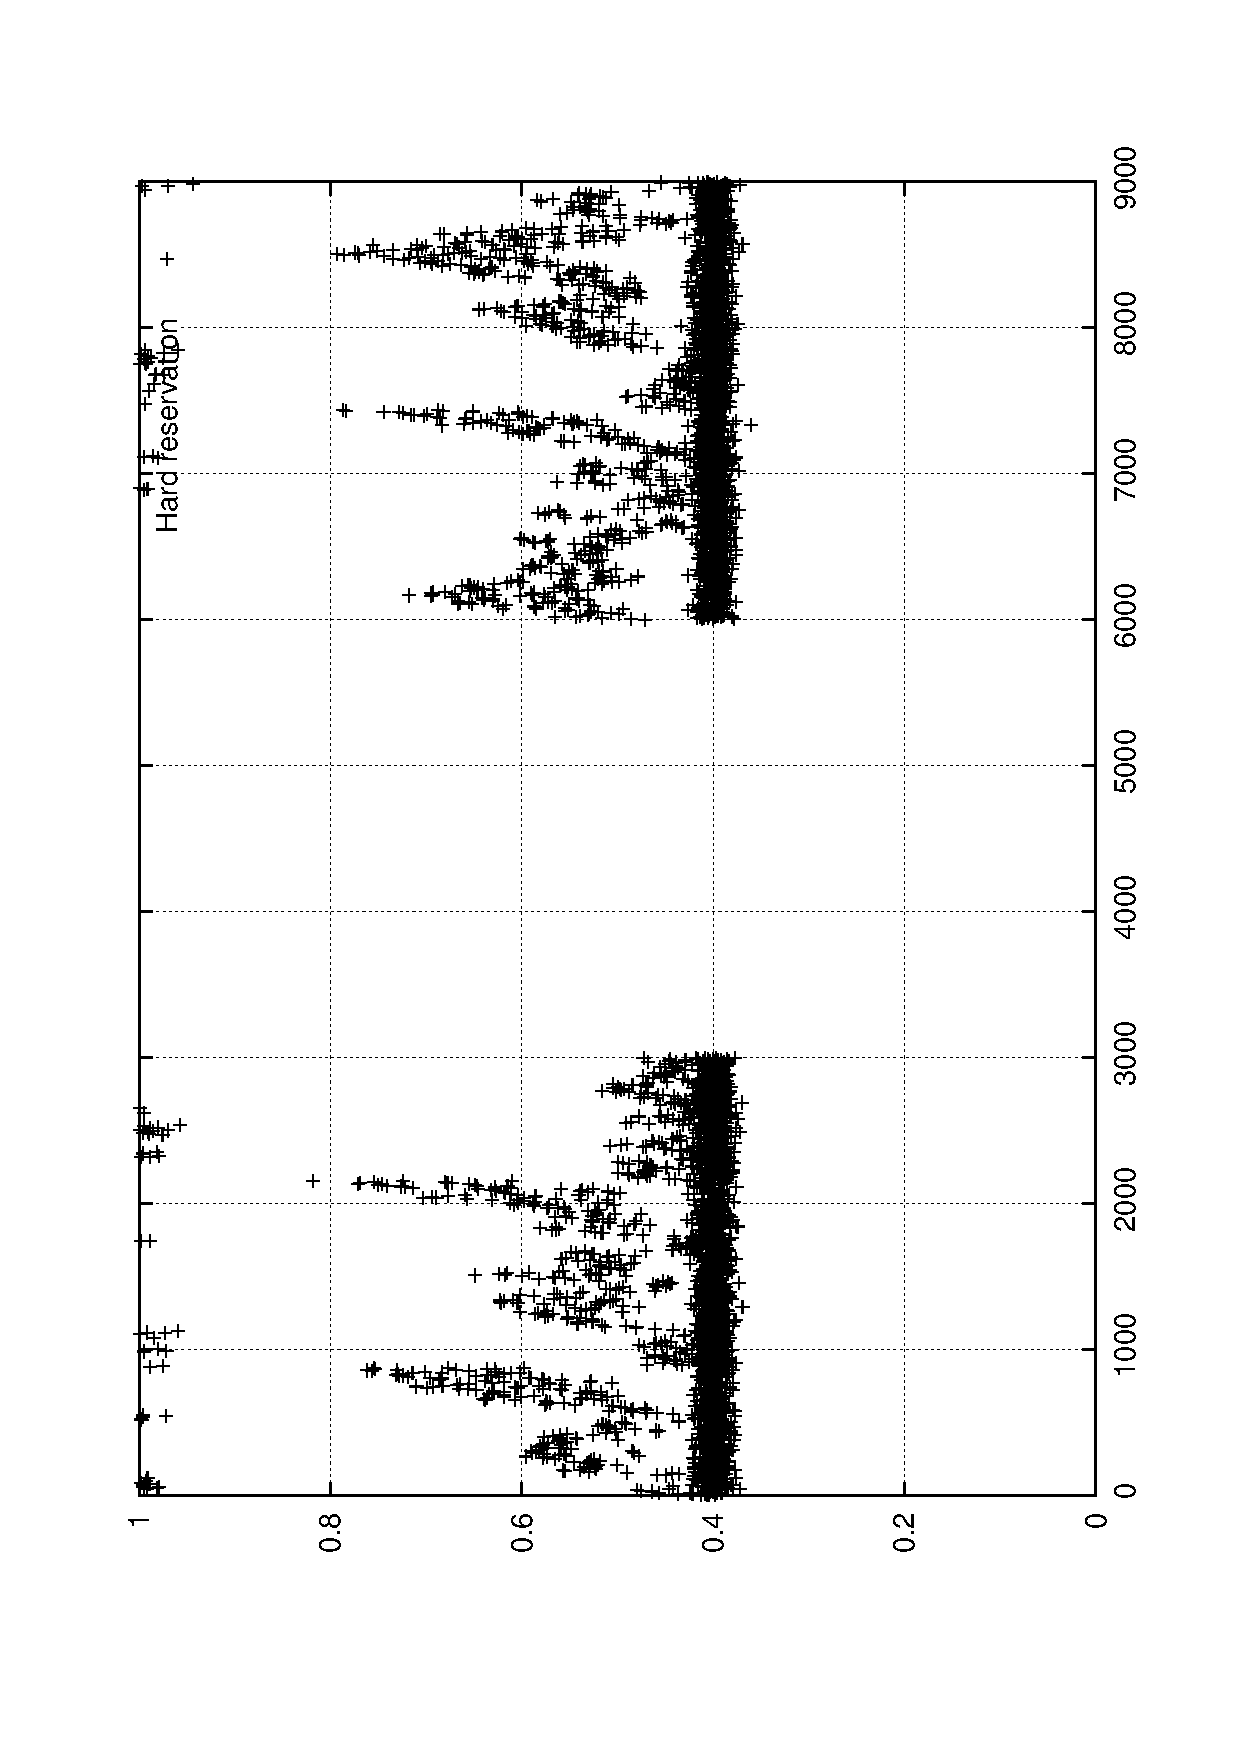
\includegraphics[scale=0.33]{trifasico-2}
    \label{fig:hard-trifasico}
  }
  \caption{Response times for scenario L2.}
  \label{fig:trifasico}
\end{figure*}

The effect of markedly different execution costs over time is also
interesting. In this experiment, the task set first starts with a
correctly dimensioned server, until a certain point in time in which
the mean costs for the tasks rise suddenly. After a while, the costs
return to normal. As can be seen in Figure \ref{fig:trifasico}, in the
heavily loaded part only the soft reservation server can finish tasks
that need more than the server budget. This might suggest that the
soft reservation server is better able to cope with run-time varying
requirements. Also, when the load comes back down there is no extra
cost for the soft reservation server, and its response times are
equivalent to the response times for the hard reservation
server. Thus, in variable environments a soft reservation scheme is
better than a hard reservation one, the latter being too brittle. This
scenario might be relevant for soft real-time systems running some
adaptation mechanism, such as the one described in
\cite{abeni.ea05:qos}.

\begin{figure*}[t]
  \centering
  \subfloat[Soft reservation.]{
    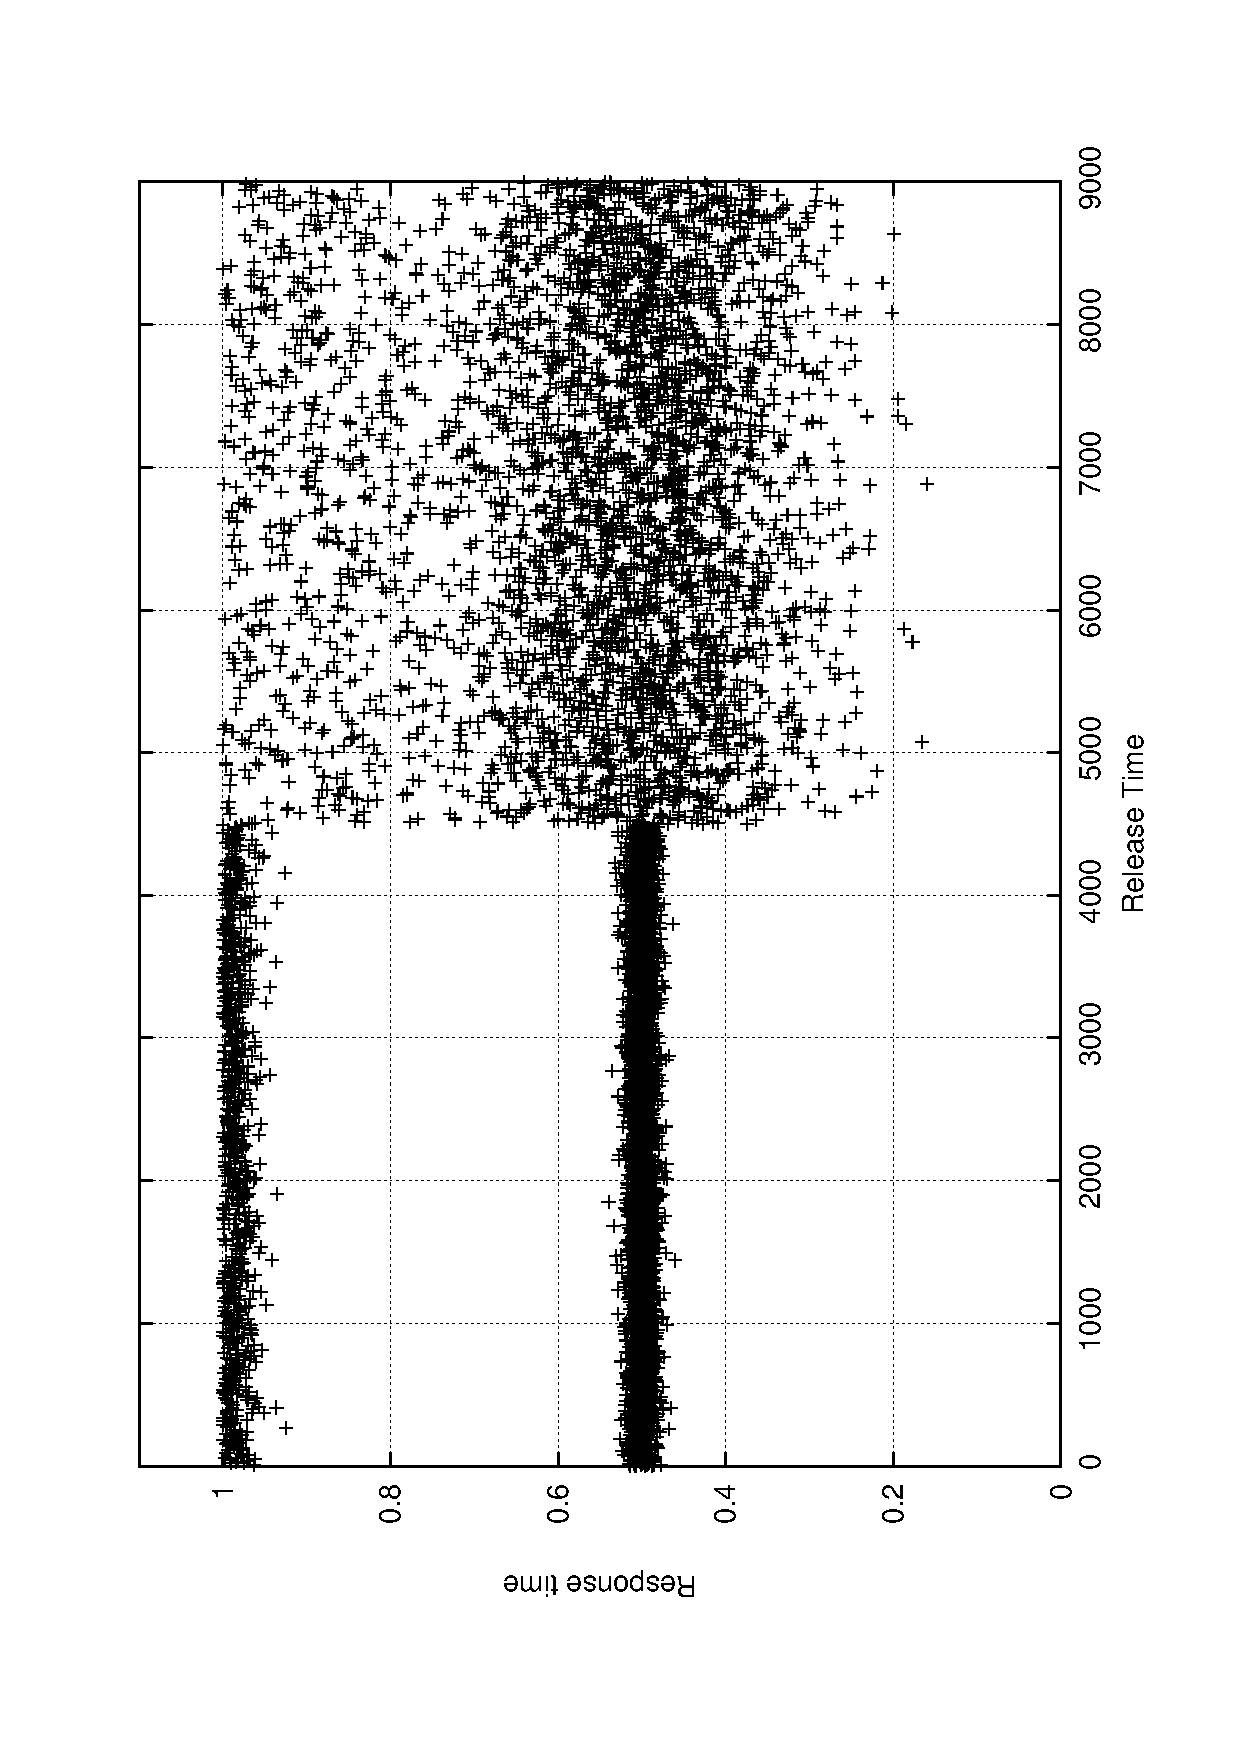
\includegraphics[scale=0.33]{variance-1}
    \label{fig:soft-variance}
  }
  \subfloat[Hard reservation.]{
    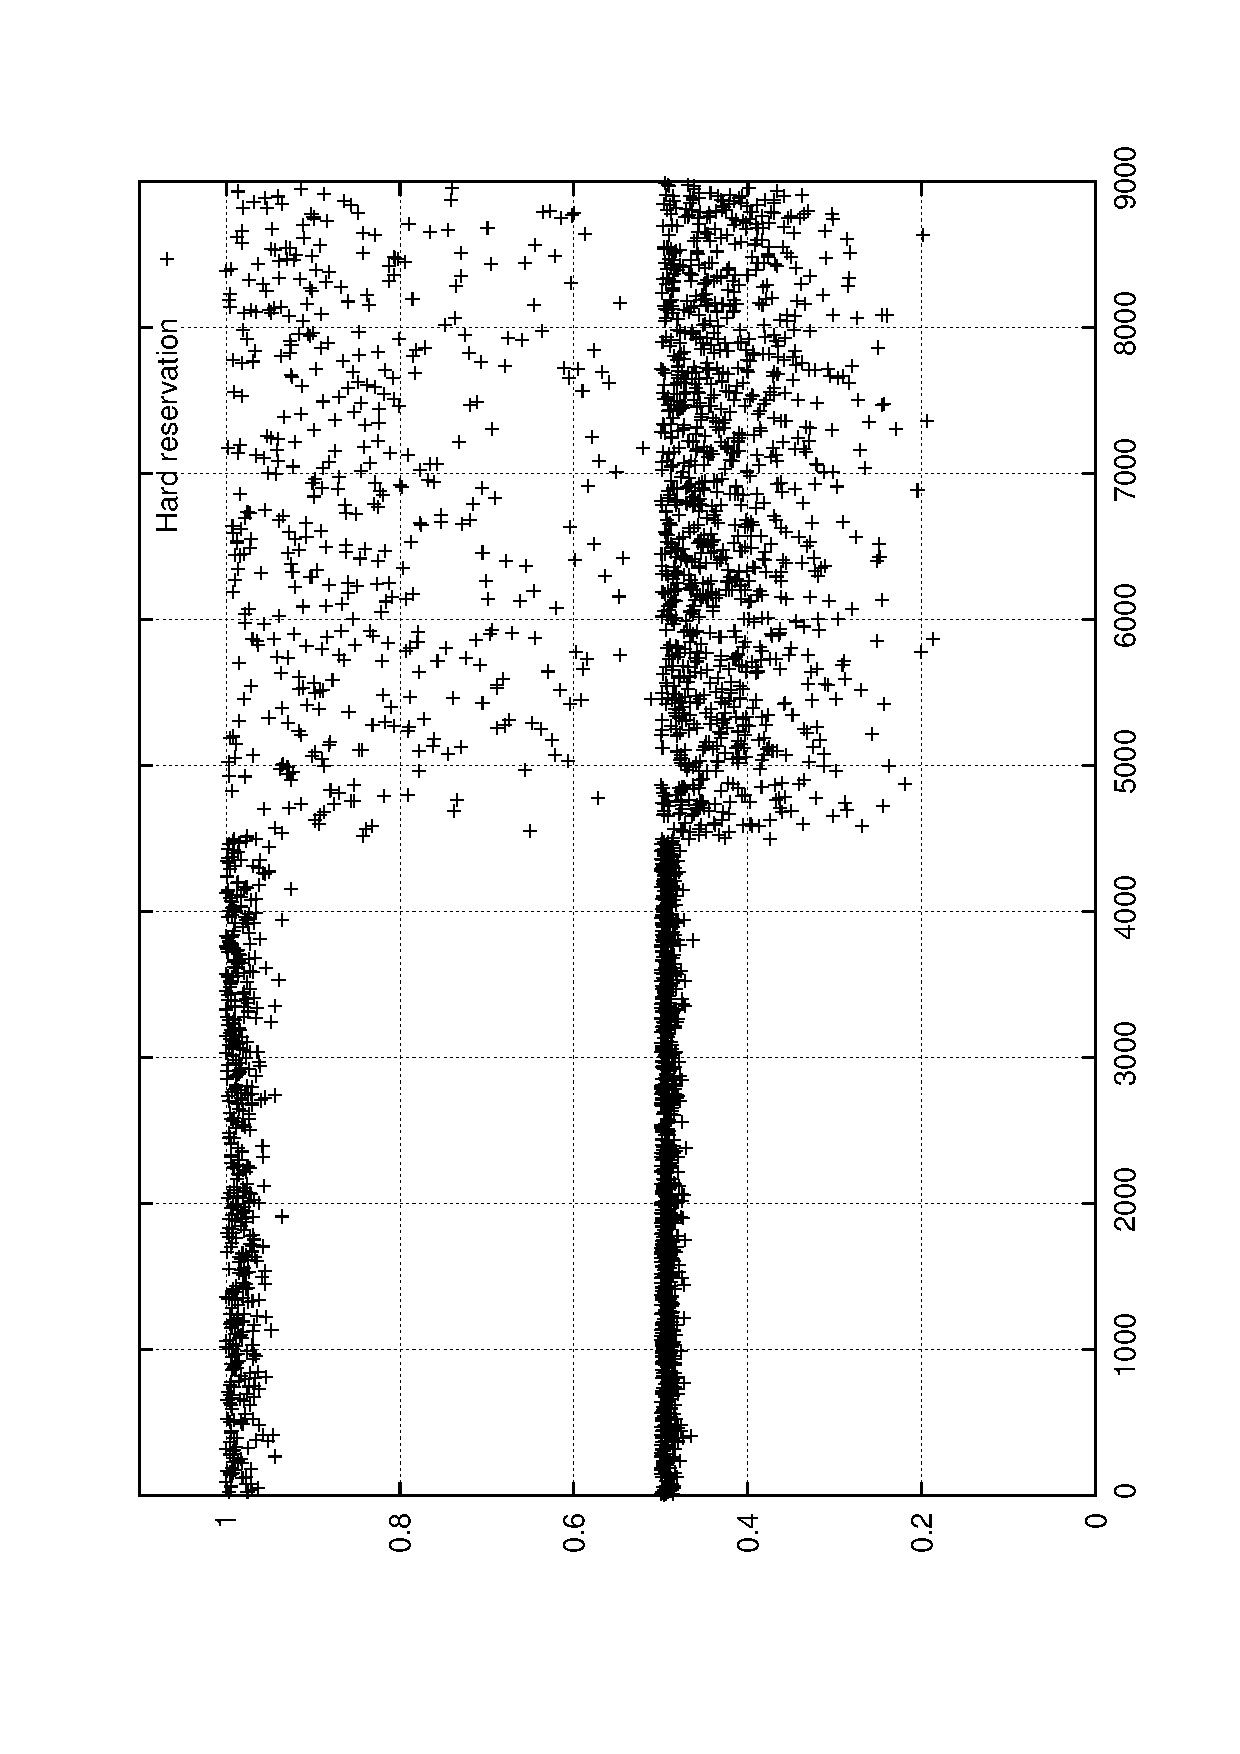
\includegraphics[scale=0.33]{variance-2}
    \label{fig:hard-variance}
  }
  \caption{Response times for scenario L3.}
  \label{fig:variance}
\end{figure*}

Another possible situation in which a RBS might have its responsivity
compromised is when dealing with tasks having a high variance in its
execution costs. Scenario L3 was designed to test this
possibility. This might happen because to serve tasks with
unexpectedly high costs, a soft reservation server might need to
postpone its deadline too much, while a hard reservation server would
be more prudent and instead discard these costly outliers, being more
performant in the remaining time. In this experiment the hard
reservation server lost 59.39\% of the deadlines, while the soft
reservation only lost 5.19\%. Figure \ref{fig:variance} shows the
response times for this experiment. As it can be easily seen, in the
higher variance part the soft reservation server manages to finish
many more tasks in a short amount of time than the hard reservation
server, thus behaving better on task sets with a high variance.

\begin{figure*}[t]
  \centering
  \subfloat[Soft reservation.]{
    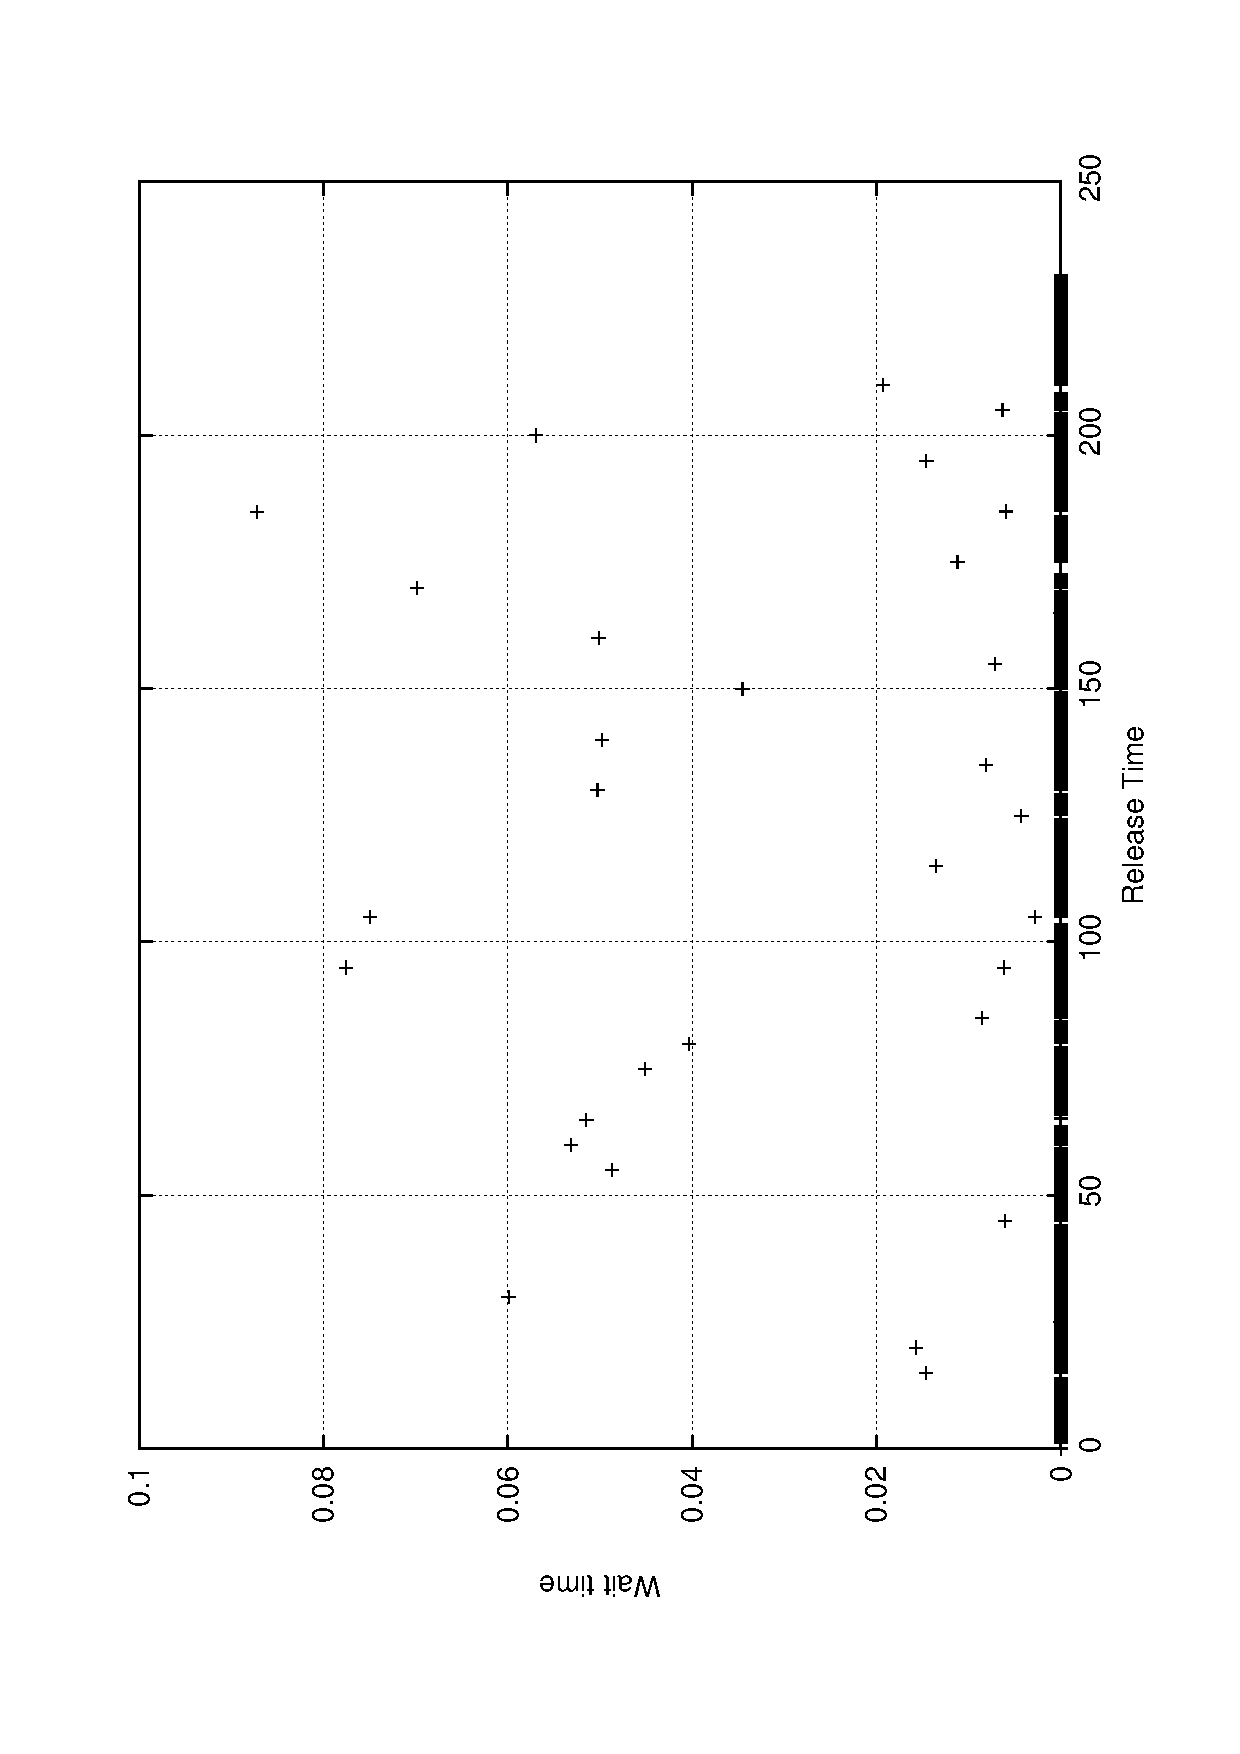
\includegraphics[scale=0.33]{eve-1}
    \label{fig:soft-eve}
  }
  \subfloat[Hard reservation.]{
    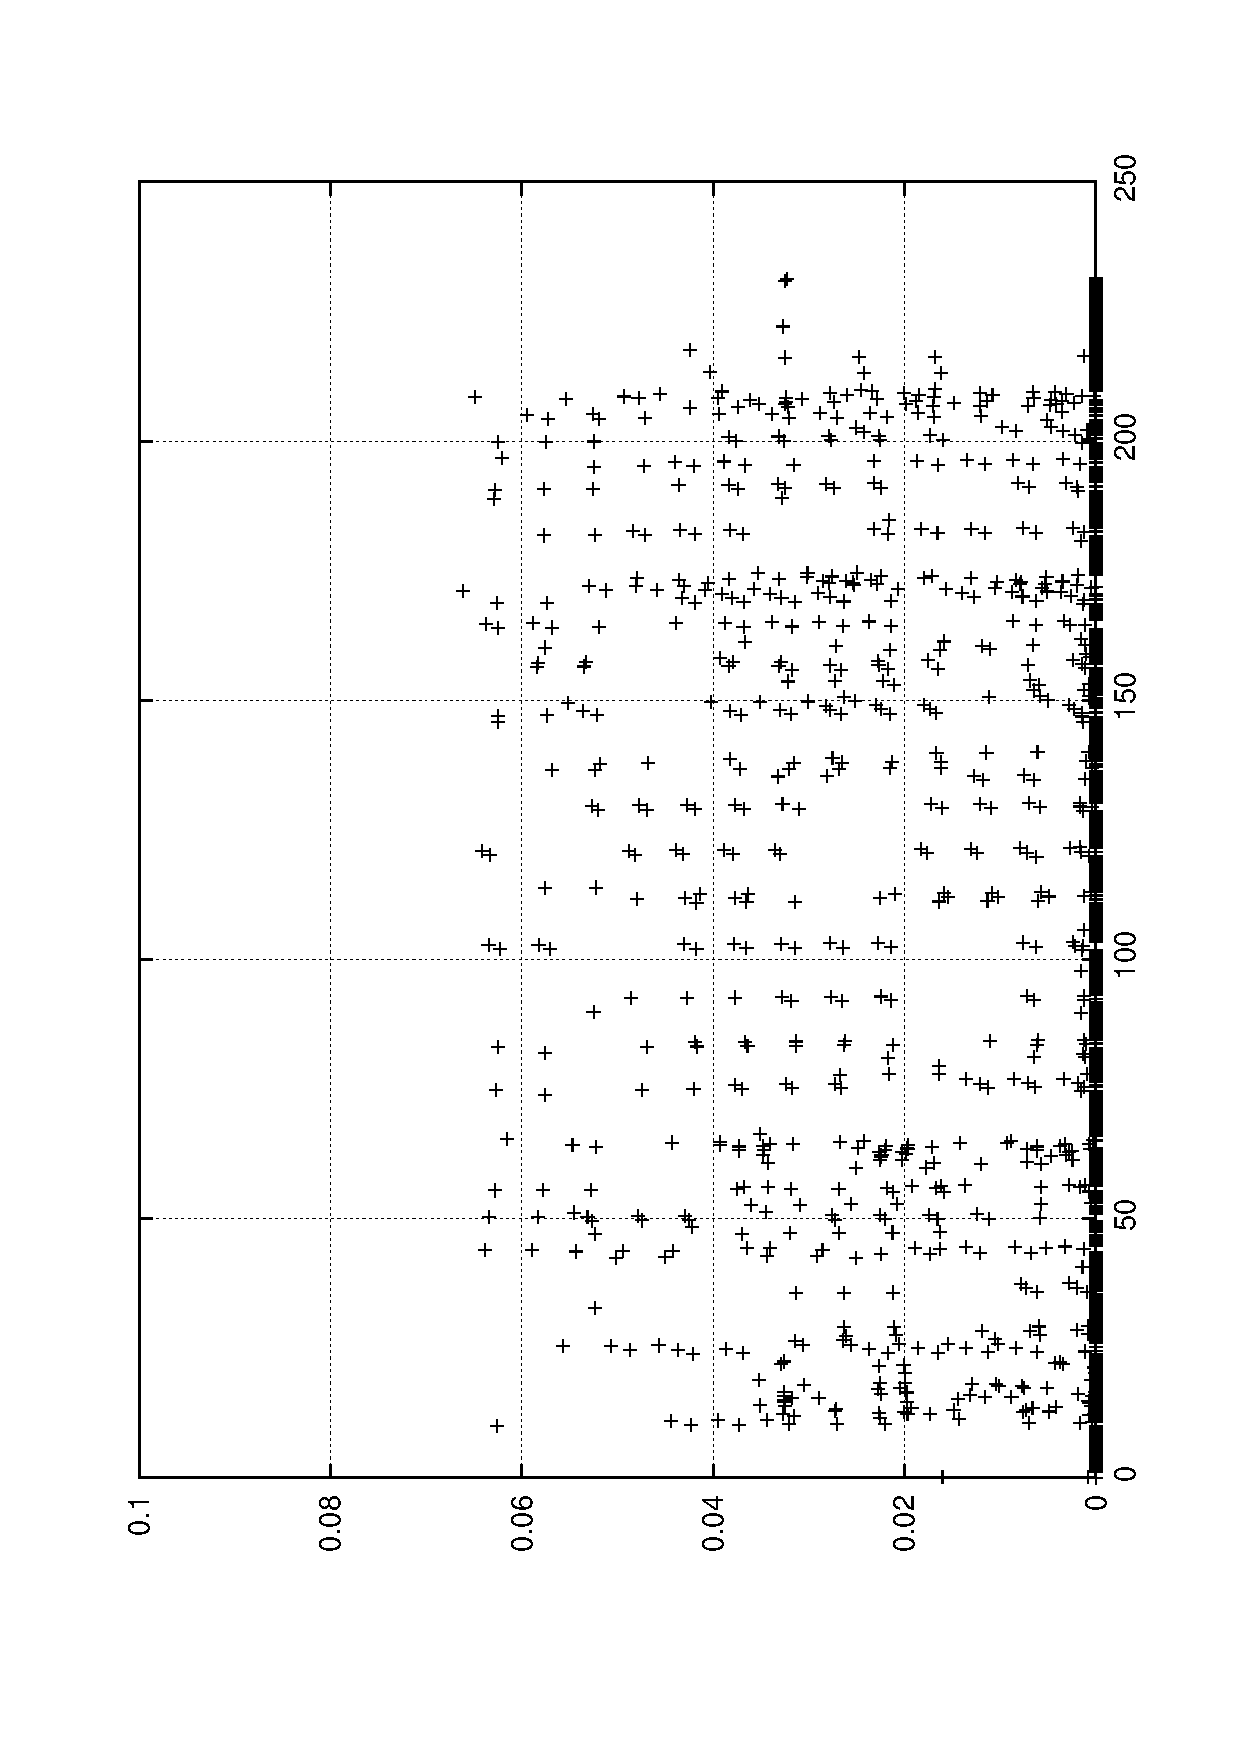
\includegraphics[scale=0.33]{eve-2}
    \label{fig:hard-eve}
  }
  \caption{Wait times for scenario L4, the movie trace.}
  \label{fig:eve}
\end{figure*}

Another very important test case is whether, in non-synthetic tasks,
the performance characteristics we observed are reproduced. In this
experiment, we ran both a soft reservation server and a hard
reservation server on scenario L4. As can be easily seen in Figure
\ref{fig:eve}, the wait time for the hard reservation server is always
higher than for the soft reservation server. Also, the soft
reservation server only lost 0.1\% of the dealines, while the hard
reservation server lost 24.54\%. This result seems, at first,
counter-intuitive, since the soft reservation server, by delaying its
deadline whenever the execution costs are too high, can have an
arbitrarily low priority. On the other hand, the same task will take
more overall time to be served with a hard reservation server, since
it will have to wait for capacity replenishment before continuing
execution.

\Section{Conclusion}
\label{sec:conclusion}

A consistently higher deadline miss ratio alone should be a warning to
users of hard reservation servers.

As can be seen in Figures \ref{fig:trifasico}, \ref{fig:variance}, and
\ref{fig:eve}, soft reservation usually outperforms hard reservation,
having a smaller average response time as well as a smaller worst-case
response time, a shorter waiting time between task arrival and start
of execution, and a more uniform interval between successive task
terminations and misses less deadlined.

\bibliographystyle{latex8}
\bibliography{bib}
\end{document}
